\section{Market power in airline markets: pricing theory}\label{sec:09-pricing}

The three empirical studies in this chapter rest on one body of pricing theory, which this section
develops in four steps. First, we derive a route-level pricing equation from a homogeneous-goods model
with a conduct parameter. This equation gives a structural reading of the fare regressions of
\cref{sec:09-borenstein}. Second, we show that airport dominance can raise a carrier's markup through
product differentiation alone, with no softening of rivals' behavior. Third, we build the finite-mixture
nested logit with $R$ consumer types that \citet{BerryCarnallSpiller2006} estimate. We derive its
shares, substitution patterns, markups and inversion. Fourth, we model costs on a network, where the
marginal cost of a passenger depends on traffic density on each flight leg, and we derive the pricing
condition of a network carrier.

Markets, carriers and products are those of \cref{sec:09-data}. A market $t$ is a directional
origin-destination pair, carriers are firms $f=1,\dots,F$, and $\mathcal{J}_t$ is the set of inside
products in market $t$. We add one piece of notation: $\mathcal{J}_f(t)\subseteq\mathcal{J}_t$ collects
the products that carrier $f$ sells in market $t$.

\subsection{From conduct to a route-level pricing equation}\label{sec:09-pricing-conduct}

We start from the simplest model that links fares to market structure. It treats travel on a route as a
homogeneous good and summarizes each carrier's behavior by a conduct parameter, as in \cref{ch:theory}
and \cref{ch:conduct}.

\begin{assumption}[Homogeneous route market]\label{ass:09-homog}
On route $t$, carriers $f=1,\dots,F$ sell a homogeneous product with outputs $q_{ft}$ and total output
$Q_t=\sum_f q_{ft}$. Inverse demand $P(Q_t)$ is differentiable and strictly decreasing, and the market
elasticity is $\varepsilon_t=-\frac{P(Q_t)}{Q_tP'(Q_t)}>0$. Carrier $f$ has constant marginal cost
$mc_{ft}$ and share $s_{ft}=\frac{q_{ft}}{Q_t}$.
\end{assumption}

\begin{definition}[Firm-level conduct]\label{def:09-conduct}
The \emph{conduct parameter} $\theta_{ft}$ of carrier $f$ on route $t$ is the number that satisfies
\begin{equation}\label{eq:09-conduct-foc}
P(Q_t)\left(1-\frac{\theta_{ft}}{\varepsilon_t}\right)=mc_{ft},
\qquad\text{equivalently}\qquad
L_{ft}\equiv\frac{P(Q_t)-mc_{ft}}{P(Q_t)}=\frac{\theta_{ft}}{\varepsilon_t}.
\end{equation}
\end{definition}

The benchmarks follow from a conjectural-variations first-order condition. Suppose carrier $f$ chooses
$q_{ft}$ and conjectures that rivals' total output $Q_{-f,t}=Q_t-q_{ft}$ responds as
$\frac{\dd Q_{-f,t}}{\dd q_{ft}}=v_{ft}$. Its first-order condition is
\begin{equation*}
P(Q_t)+q_{ft}P'(Q_t)\,(1+v_{ft})-mc_{ft}=0 .
\end{equation*}
Dividing by $P(Q_t)$ and using the definitions of $s_{ft}$ and $\varepsilon_t$,
\begin{equation*}
\frac{P-mc_{ft}}{P}
=-\frac{q_{ft}P'(Q_t)}{P}\,(1+v_{ft})
=\frac{q_{ft}}{Q_t}\left(-\frac{Q_tP'(Q_t)}{P}\right)(1+v_{ft})
=\frac{s_{ft}(1+v_{ft})}{\varepsilon_t}.
\end{equation*}
Hence $\theta_{ft}=s_{ft}(1+v_{ft})$. Cournot conjectures ($v_{ft}=0$) give $\theta_{ft}=s_{ft}$, which
equals $\frac{1}{N}$ with $N$ symmetric firms. Price taking gives $\theta_{ft}=0$. When all carriers have
the same cost, joint profit maximization sets $\frac{P-mc}{P}=\frac{1}{\varepsilon_t}$, so
$\theta_{ft}=1$.

We parametrize conduct between Cournot and joint profit maximization as
\begin{equation}\label{eq:09-theta-param}
\theta_{ft}=s_{ft}+\eta_t\,(1-s_{ft}),\qquad \eta_t\in[0,1].
\end{equation}
Matching $\theta_{ft}=s_{ft}(1+v_{ft})$ gives $v_{ft}=\eta_t\frac{1-s_{ft}}{s_{ft}}=\eta_t\frac{Q_{-f,t}}{q_{ft}}$,
which rearranges to $\frac{\dd Q_{-f,t}}{Q_{-f,t}}=\eta_t\frac{\dd q_{ft}}{q_{ft}}$. Carrier $f$ therefore
expects rivals to change their output by $\eta_t$ percent when it changes its own by one percent. We call
$\eta_t$ the \emph{collusiveness} of route $t$. With $\eta_t=0$ carriers play Cournot, and with
$\eta_t=1$ every carrier prices as a joint monopolist would.

\casehead{The pricing equation}
Write $p_t=P(Q_t)$ for the route price and take logs of \eqref{eq:09-conduct-foc}:
\begin{equation*}
\ln p_t=\ln mc_{ft}-\ln\left(1-\frac{\theta_{ft}}{\varepsilon_t}\right).
\end{equation*}
The expansion $-\ln(1-x)=x+\frac{x^2}{2}+\frac{x^3}{3}+\cdots$ gives $-\ln(1-x)\approx x$ when
$x=\frac{\theta_{ft}}{\varepsilon_t}$ is small, so
\begin{equation*}
\ln p_t\approx\ln mc_{ft}+\frac{\theta_{ft}}{\varepsilon_t}.
\end{equation*}
Substituting \eqref{eq:09-theta-param},
\begin{align}
\ln p_t&\approx\ln mc_{ft}+\frac{s_{ft}+\eta_t(1-s_{ft})}{\varepsilon_t}\notag\\
&=\ln mc_{ft}+\frac{\eta_t}{\varepsilon_t}+\frac{1-\eta_t}{\varepsilon_t}\,s_{ft}.
\label{eq:09-pricing-approx}
\end{align}
The approximation is accurate for moderate Lerner indices. At $\frac{\theta_{ft}}{\varepsilon_t}=0.2$ the
exact term is $-\ln 0.8=0.223$, against $0.2$ for the linear term, so the linear form slightly understates
large markups.

Equation \eqref{eq:09-pricing-approx} splits the log price into three parts. The first is marginal cost.
The second, $\frac{\eta_t}{\varepsilon_t}$, is a route-level markup shared by every carrier. The third is
an own-share term with slope $\frac{1-\eta_t}{\varepsilon_t}$. Under Cournot conduct the slope is
$\frac{1}{\varepsilon_t}$ and the route-level term vanishes. Under joint profit maximization the slope is
zero, and every carrier's markup reflects only $\frac{1}{\varepsilon_t}$. The share coefficient therefore
falls as conduct becomes more collusive.

\casehead{The umbrella hypothesis}
The \emph{umbrella hypothesis} holds that a dominant carrier's high fares shelter its smaller rivals,
which can then price above their competitive level. A natural way to formalize it is to let concentration
raise collusiveness,
\begin{equation}\label{eq:09-umbrella-eta}
\eta_t=\eta_0+\eta_1\HHI_t,\qquad \eta_1>0,
\end{equation}
where $\HHI_t=\sum_f s_{ft}^2$ is the route Herfindahl index. Substituting \eqref{eq:09-umbrella-eta}
into \eqref{eq:09-pricing-approx} and collecting terms,
\begin{align}
\ln p_t&\approx\ln mc_{ft}+\frac{\eta_0+\eta_1\HHI_t}{\varepsilon_t}
+\frac{1-\eta_0-\eta_1\HHI_t}{\varepsilon_t}\,s_{ft}\notag\\
&=\ln mc_{ft}+\frac{\eta_0}{\varepsilon_t}+\frac{1-\eta_0}{\varepsilon_t}\,s_{ft}
+\frac{\eta_1}{\varepsilon_t}\,\HHI_t-\frac{\eta_1}{\varepsilon_t}\,\HHI_t\,s_{ft}.
\label{eq:09-umbrella}
\end{align}
The effect of concentration on a carrier's price is
$\frac{\partial\ln p_t}{\partial\HHI_t}=\frac{\eta_1(1-s_{ft})}{\varepsilon_t}$. It is largest for the
carriers with the smallest shares, which is exactly what an umbrella means.

Equation \eqref{eq:09-umbrella} maps into the market-power block of Borenstein's pricing equation
\eqref{eq:09-bor-price}, which omits the interaction $\HHI_t\,s_{ft}$. Let $\bar H$ and $\bar s$ be the
sample means of $\HHI_t$ and $s_{ft}$. Linearizing the interaction around them gives
$\HHI_ts_{ft}\approx\bar H s_{ft}+\bar s\HHI_t-\bar s\bar H$. Holding the elasticity fixed, the
route-share coefficient (RUTSHARE) is then $\phi_3\approx\frac{1-\eta_0-\eta_1\bar H}{\varepsilon}$. The
route-Herfindahl coefficient (RUTHERF) is $\phi_4\approx\frac{\eta_1(1-\bar s)}{\varepsilon}$. The
umbrella hypothesis still predicts $\phi_4>0$, and $\eta_1=0$ still gives $\phi_4=0$. In Borenstein's
sample $\bar H=0.50$ and $\bar s=0.54$ \citep[Table~4]{Borenstein1989}, so $\phi_4$ is less than half of
$\frac{\eta_1}{\varepsilon}$. Variation in $\varepsilon_t$ across routes makes all three coefficients
averages as well, which is one reason to control for the tourist share of a route's travelers.

\casehead{Share-weighted margins}
Multiplying the Lerner index $L_{ft}=\frac{\theta_{ft}}{\varepsilon_t}$ by $s_{ft}$ and summing over
carriers gives the route's share-weighted margin:
\begin{align}
\sum_f s_{ft}L_{ft}
&=\frac{1}{\varepsilon_t}\sum_f s_{ft}\big[s_{ft}+\eta_t(1-s_{ft})\big]
=\frac{1}{\varepsilon_t}\Big[\sum_f s_{ft}^2+\eta_t\Big(\sum_f s_{ft}-\sum_f s_{ft}^2\Big)\Big]\notag\\
&=\frac{(1-\eta_t)\HHI_t+\eta_t}{\varepsilon_t}.\label{eq:09-cowling}
\end{align}
With $\eta_t=0$ this is the result $\frac{\HHI_t}{\varepsilon_t}$ of \citet{CowlingWaterson1976}
(\cref{prop:02-cowling-waterson}). Under Cournot conduct, share-weighted margins rise with concentration even when
conduct is identical on every route. A cross-route regression of margins on $\HHI_t$ in the
structure-conduct-performance tradition (\cref{ch:intro}) therefore finds a positive slope without any
umbrella effect. Under joint profit maximization ($\eta_t=1$) the share-weighted margin is
$\frac{1}{\varepsilon_t}$ whatever the concentration.

\casehead{Functional form}
Equation \eqref{eq:09-pricing-approx} explains the functional form that the airline pricing literature
adopted. Profit maximization makes price proportional to marginal cost times an inverse-elasticity term,
so the cost part enters in logs \citep[p.~354]{Borenstein1989}. Borenstein parametrizes $\ln mc_{ft}$
by a carrier effect, the log of nonstop distance and logs of cost and quality variables such as load
factor, aircraft size, frequency and circuity. Shares and Herfindahl indices enter linearly. Borenstein
motivates the linear share with an example \citep[p.~354]{Borenstein1989}. A rise in share from 1\% to 2\%
should not have the same effect as a rise from 30\% to 60\%. Our derivation adds a theoretical reason: to
first order, the log price is linear in the share. \citet{BaileyGrahamKaplan1985} had already included the observed carrier's route share and found a
positive effect after controlling for route concentration \citep[p.~348, n.~18]{Borenstein1989}.
Borenstein describes his equation as a supply relation in the framework of \citet{Bresnahan1989}. The cost function is never estimated separately. It is
inferred from cross-sectional variation in prices and product attributes \citep[p.~348, n.~18]{Borenstein1989},
as in \cref{ch:conduct}.

\begin{remark}[What the share coefficient can and cannot reveal]\label{rem:09-share-coef}
Borenstein's \emph{two-stage least squares} (2SLS) estimates of $\phi_3$ range from $0.029$ for the median fare to
$0.224$ for the 80th percentile fare \citep[Table~2]{Borenstein1989}. Equation
\eqref{eq:09-umbrella} reads these numbers as $\frac{1-\bar\eta}{\varepsilon}$, where
$\bar\eta=\eta_0+\eta_1\bar H$ is the collusiveness at the mean Herfindahl index. A Cournot reading
with $\bar\eta=0$ requires market elasticities $\varepsilon=\frac{1}{\phi_3}$ between about $4.5$ and
$35$. A market elasticity of $1.5$ instead requires $\bar\eta=1-1.5\,\phi_3$, between $0.66$ and $0.96$,
which is close to joint profit maximization. Small share coefficients are thus consistent either with
elastic route demand or with nearly collusive conduct. Without an independent estimate of $\varepsilon$
the regression cannot tell the two apart. This is the identification problem of \cref{ch:conduct} in a
new setting.
\end{remark}

Two features of airline markets strain the homogeneous-goods model and motivate the rest of this section.
First, the model predicts a single price on each route. Carriers on the same route charge different
fares, and each sells many fares. Borenstein's relative-price equation \eqref{eq:09-bor-rel} compares two
carriers' fares on the same route, and in the homogeneous model its left side is identically zero. With
a common price, \eqref{eq:09-pricing-approx} also forces carriers with larger shares to have lower
marginal costs. Second, a large share may reflect a better product or a lower cost rather than market
power. \citet{Demsetz1973} made this argument for concentration across industries (\cref{ch:intro}).
In the homogeneous model the share is a sufficient statistic for cost efficiency. When costs are measured
with error, the share coefficient absorbs the unmeasured part of cost. In a differentiated market, a
carrier with a more attractive product has both a larger share and a higher price, so the share
coefficient also absorbs quality. Instruments for the share, such as Borenstein's GENPSH
(\cref{sec:09-borenstein}), address the simultaneity of share and price. They cannot separate market
power from quality when the two are the same thing, as the next model shows.

\subsection{Dominance as product differentiation: markups without an umbrella}\label{sec:09-pricing-diff}

Many of the sources of airport dominance described in \cref{sec:09-dominance-sources} work through
demand.
A frequent-flyer program is worth more when the carrier flies to more places from the traveler's home
airport. Frequency, convenient gates and a local reputation make a carrier's flights more attractive.
\citet{Berry1990} treats airport presence as a source of product differentiation in this sense. We now model
dominance as higher non-price quality and ask what it implies for prices.

\begin{assumption}[Logit route market]\label{ass:09-logit}
Route $t$ (subscript dropped) has single-product carriers $j=1,\dots,J$ and an outside good $j=0$.
Consumer $i$ has utility $u_{ij}=\delta_j-\alpha p_j+\epsilon_{ij}$ for $j\ge1$ and $u_{i0}=\epsilon_{i0}$,
with $\epsilon_{ij}$ i.i.d.\ type-I extreme value and $\alpha>0$. Carrier $j$ has constant marginal cost
$c_j$ and chooses $p_j$ to maximize $(p_j-c_j)Ms_j(p)$, taking rivals' prices as given.
\end{assumption}

In this subsection only, $\delta_j$ denotes the non-price part of mean utility ($x_j\beta+\xi_j$ in the
notation of \cref{ch:logit}), so that mean utility including price is $\delta_j-\alpha p_j$. Shares and
own-price derivatives are (\cref{ch:logit})
\begin{equation*}
s_j=\frac{e^{\delta_j-\alpha p_j}}{1+\sum_{k=1}^J e^{\delta_k-\alpha p_k}},
\qquad
\frac{\partial s_j}{\partial p_j}=-\alpha s_j(1-s_j).
\end{equation*}
The first-order condition $s_j+(p_j-c_j)\frac{\partial s_j}{\partial p_j}=0$ becomes
$s_j-\alpha(p_j-c_j)s_j(1-s_j)=0$. Dividing by $\alpha s_j(1-s_j)$,
\begin{equation}\label{eq:09-logit-markup}
p_j-c_j=\frac{1}{\alpha(1-s_j)} .
\end{equation}

\begin{proposition}[Dominance without an umbrella]\label{prop:09-dominance}
Under \cref{ass:09-logit} the Bertrand-Nash equilibrium exists and is unique. In equilibrium:
\begin{enumerate}[label=(\roman*)]
\item Each carrier's markup $p_j-c_j=\frac{1}{\alpha(1-s_j)}$ is strictly increasing in its own share, so
carriers with larger shares charge larger markups.
\item An increase in $\delta_1$ raises $p_1$ and $s_1$, lowers the outside share $s_0$, and lowers $p_k$
and $s_k$ for every rival $k\neq1$.
\end{enumerate}
\end{proposition}

\begin{proof}
Part (i) is immediate from \eqref{eq:09-logit-markup}. For part (ii) and for existence and uniqueness we
reduce the equilibrium to a single equation in $s_0$.

\emph{Step 1 (one equation per carrier).} Let $m_j=p_j-c_j$ and $a_j=e^{\delta_j-\alpha c_j}$. The
first-order condition \eqref{eq:09-logit-markup} is $s_j=1-\frac{1}{\alpha m_j}$, which requires
$m_j>\frac{1}{\alpha}$. The logit formula gives
$\frac{s_j}{s_0}=e^{\delta_j-\alpha p_j}=a_je^{-\alpha m_j}$. Substituting the first-order condition
into the logit ratio,
\begin{equation*}
1-\frac{1}{\alpha m_j}=s_0\,a_je^{-\alpha m_j},
\qquad\text{so}\qquad
h(m_j)\equiv\Big(1-\frac{1}{\alpha m_j}\Big)e^{\alpha m_j}=s_0\,a_j .
\end{equation*}

\emph{Step 2 ($h$ is invertible).} On $\big(\frac{1}{\alpha},\infty\big)$, $h$ is continuous, $h$ tends
to $0$ as $m\downarrow\frac{1}{\alpha}$, and $h(m)\to\infty$ as $m\to\infty$. Its derivative is
\begin{equation*}
h'(m)=e^{\alpha m}\Big[\frac{1}{\alpha m^2}+\alpha-\frac{1}{m}\Big]
=e^{\alpha m}\,\frac{(\alpha m)^2-\alpha m+1}{\alpha m^2}>0,
\end{equation*}
because $x^2-x+1=\big(x-\frac{1}{2}\big)^2+\frac{3}{4}>0$. Hence $m_j=h^{-1}(s_0a_j)$ is strictly
increasing in $s_0a_j$. The share is $s_j=S(s_0a_j)$ with
$S(y)\equiv1-\frac{1}{\alpha h^{-1}(y)}$, which is continuous and strictly increasing, with $S(y)\to0$ as
$y\to0$ and $S(y)\to1$ as $y\to\infty$.

\emph{Step 3 (existence and uniqueness).} Shares add up to one:
\begin{equation*}
G(s_0;a)\equiv s_0+\sum_{j=1}^J S(s_0a_j)=1 .
\end{equation*}
$G$ is continuous and strictly increasing in $s_0$, with $G(0;a)=0$ and $G(1;a)>1$. A unique
$s_0^*\in(0,1)$ solves the equation, and Step 2 then gives unique markups and shares. Any equilibrium
satisfies the first-order conditions, so there is at most one equilibrium. The first-order conditions
are also sufficient. Given rivals' prices, the left side of $p_j-c_j=\frac{1}{\alpha(1-s_j(p))}$ rises in
$p_j$ while the right side falls, because $s_j$ falls in $p_j$. Profit therefore rises below the unique
crossing and falls above it, so the crossing is the best response.

\emph{Step 4 (comparative statics).} A higher $\delta_1$ raises $a_1$. Since $S$ is increasing,
$G(s_0;a)$ rises at every $s_0$, so the solution $s_0^*$ falls. For each $k\neq1$, the product
$s_0^*a_k$ falls, so $m_k$ and $s_k$ fall, and $p_k=c_k+m_k$ falls. Finally
$s_1=1-s_0^*-\sum_{k\neq1}s_k$ rises because $s_0^*$ and every $s_k$ fall. Then
$m_1=\frac{1}{\alpha(1-s_1)}$ rises and so does $p_1=c_1+m_1$.
\end{proof}

The existence and uniqueness result agrees with the general results for logit-type demand in
\cref{ch:diffprod} \citep{CaplinNalebuff1991}. The single-equation reduction is useful in its own right,
since it computes the equilibrium by solving one monotone equation. \Cref{fig:09-dominance} uses it.

\begin{figure}[htbp]
\centering
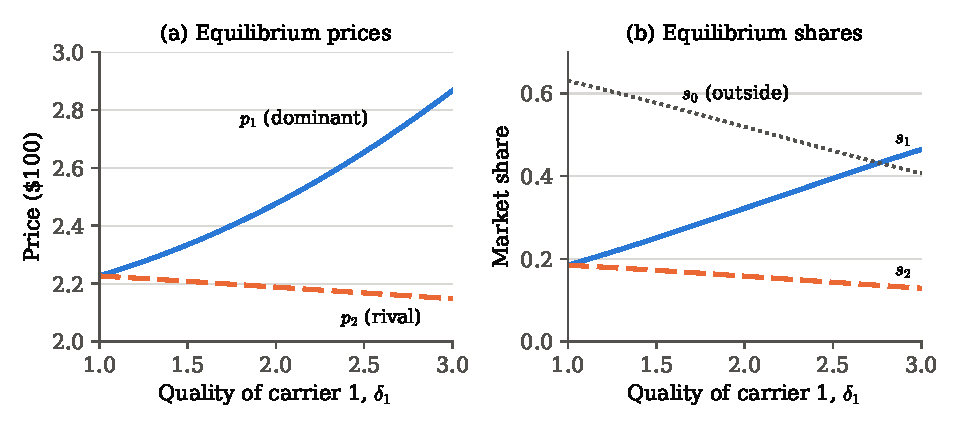
\includegraphics[width=\textwidth]{figures/ch09/logit_dominance.pdf}
\caption{Logit Bertrand equilibrium on a route with two carriers and an outside good, as carrier 1's
non-price quality $\delta_1$ rises. Parameters are $\alpha=1$ (prices in \$100), $c_1=c_2=1$ and
$\delta_2=1$. At $\delta_1=1$ both carriers charge $2.227$. At $\delta_1=3$, $p_1=2.867$, $p_2=2.148$,
$s_1=0.464$ and $s_2=0.129$. The dominant carrier's price rises while its rival's falls.}
\label{fig:09-dominance}
\end{figure}

\Cref{fig:09-dominance} traces the equilibrium of a two-carrier route as carrier 1's quality rises from
$\delta_1=1$ to $\delta_1=3$. Carrier 1's share rises from $0.185$ to $0.464$ and its price from $2.227$
to $2.867$. The rival's share falls from $0.185$ to $0.129$ and its price from $2.227$ to $2.148$.
The Herfindahl index of inside shares rises from $0.500$ to $0.660$. Concentration rises and the rival's
price falls, the opposite of an umbrella. Logit prices are strategic complements, so carrier 1's higher
price alone would push $p_2$ up. The loss of customers to the better product outweighs this effect, and
the rival's markup $\frac{1}{\alpha(1-s_2)}$ falls with its share.

\begin{corollary}[Relative prices]\label{cor:09-relprice}
Under \cref{ass:09-logit}, an increase in $\delta_1$ raises $\ln p_1-\ln p_k$ for every $k\neq1$. Along
any path of shares, $\frac{\dd\ln p_j}{\dd s_j}=\frac{L_j}{1-s_j}$, where $L_j=\frac{p_j-c_j}{p_j}$ is
the Lerner index. With equal costs, $\ln p_1-\ln p_k\approx\frac{L}{1-s}\,(s_1-s_k)$ for shares near a
common value $s$ with Lerner index $L$.
\end{corollary}

\begin{proof}
The first claim follows from \cref{prop:09-dominance}(ii), since $p_1$ rises and $p_k$ falls. For the
slope, differentiate \eqref{eq:09-logit-markup}:
$\frac{\dd m_j}{\dd s_j}=\frac{1}{\alpha(1-s_j)^2}=\frac{m_j}{1-s_j}$. Then
$\frac{\dd\ln p_j}{\dd s_j}=\frac{1}{p_j}\frac{\dd m_j}{\dd s_j}=\frac{m_j}{p_j}\frac{1}{1-s_j}=\frac{L_j}{1-s_j}$.
A first-order expansion around the common share gives the approximation.
\end{proof}

The corollary is the structural counterpart of Borenstein's relative-price equation
\eqref{eq:09-bor-rel}. There, the coefficient on the difference in route shares between two carriers on
the same route plays the role of $\frac{L(1-s_0)}{1-s}$. Route shares are shares of fliers,
$\frac{s_j}{1-s_0}$, so the gap in route shares between carriers 1 and $k$ is $\frac{s_1-s_k}{1-s_0}$.
A positive coefficient is what product differentiation
predicts, with no change in conduct. In the example of \cref{fig:09-dominance}, $\ln p_1-\ln p_2$ rises
from $0$ to $0.289$ as $\delta_1$ goes from 1 to 3.

\begin{remark}[Quality or cost?]\label{rem:09-quality-cost}
The equilibrium depends on $(\delta_j,c_j)$ only through $a_j=e^{\delta_j-\alpha c_j}$. A cost advantage
therefore has the same effect on shares and markups as a quality advantage of $\alpha$ times the cost
gap. In the example of \cref{fig:09-dominance}, $(\delta_1,c_1)=(1.5,1)$ and $(\delta_1,c_1)=(1,0.5)$
give identical shares ($s_1=0.251$, $s_2=0.172$) and the same markup $m_1=1.334$. Only carrier 1's price
differs, $2.334$ against $1.834$. A relation between shares and markups cannot reveal whether dominance
comes from quality or from cost. Separating them requires a model of costs, which is what
\cref{sec:09-pricing-network} and \cref{sec:09-bcs} provide.
\end{remark}

\casehead{Multi-product carriers}
A carrier usually sells several products on a route: direct and connecting itineraries, and several fare
classes. With logit demand, the first-order condition for $j\in\mathcal{J}_f$ is
$s_j-\alpha s_jm_j+\alpha s_j\sum_{k\in\mathcal{J}_f}s_km_k=0$. Dividing by $\alpha s_j$ gives
$m_j=\frac{1}{\alpha}+\sum_{k\in\mathcal{J}_f}s_km_k$. The right side does not depend on $j$, so all of
the carrier's products carry a common markup $m_f$. Substituting back,
$m_f=\frac{1}{\alpha}+S_fm_f$, so
\begin{equation*}
m_f=\frac{1}{\alpha(1-S_f)},\qquad S_f=\sum_{k\in\mathcal{J}_f}s_k
\end{equation*}
(\cref{ch:logit}). Summing the logit ratios over the carrier's products gives
$\frac{S_f}{s_0}=A_fe^{-\alpha m_f}$ with $A_f=\sum_{k\in\mathcal{J}_f}a_k$. The proof of
\cref{prop:09-dominance} then applies with carriers in place of products and $A_f$ in place of $a_j$.
A carrier with a large total share on the route earns a large markup on every product it sells there.

The logit model also has a limitation that matters for airlines. Every product of a carrier carries the
same dollar markup, whether it is a restricted discount ticket or an unrestricted fare. Characteristics
affect the markup only through shares. The model cannot express the idea that a hub lets its carrier
raise fares mainly to business travelers. That requires heterogeneity in price sensitivity, to which we
now turn.

\subsection{Consumer heterogeneity: a finite-mixture nested logit}\label{sec:09-pricing-types}

Air travelers differ in ways that matter for pricing. Business travelers are less sensitive to price
\citep[p.~10, n.~9]{BerryCarnallSpiller2006}. Their trips are urgent, travel is a deductible business
expense, and the traveler may not bear the full cost of the ticket. They may also value frequency, nonstop service and
frequent-flyer benefits more, so tastes are correlated across characteristics. A model in which the
price coefficient and the tastes vary across consumers lets markups differ across the products of one
carrier. It also lets a hub's demand advantage fall on particular travelers.
Earlier discrete choice models of air travel, such as that of \citet{MorrisonWinston1986}, used a
logit with common coefficients \citep[p.~8]{BerryCarnallSpiller2006}. \citet{BerryCarnallSpiller2006}
adopt the simplest distribution with heterogeneous tastes, a two-point distribution of types. We develop the model with $R$ types and specialize to $R=2$ in \cref{sec:09-bcs}.

\begin{assumption}[Finite-mixture nested logit]\label{ass:09-fm}
Market $t$ has $M_t$ potential travelers. Each belongs to one of $R$ types, and type $r$ has population
share $\psi_r>0$ with $\sum_r\psi_r=1$. A traveler $i$ of type $r$ has utility
\begin{equation*}
u_{ijt}=x_{jt}\beta_r-\alpha_rp_{jt}+\xi_{jt}+\zeta_{igt}+(1-\sigma)\epsilon_{ijt}
\quad (j\in\mathcal{J}_t),\qquad u_{i0t}=\epsilon_{i0t}.
\end{equation*}
The shocks $\epsilon_{ijt}$ are i.i.d.\ type-I extreme value. All inside goods form one nest $g$ and the
outside good forms its own nest. The term $\zeta_{igt}$ is common to all inside goods for traveler $i$
and has the distribution of \citet{Cardell1997}, which makes $\zeta_{igt}+(1-\sigma)\epsilon_{ijt}$
type-I extreme value, with $\sigma\in[0,1)$. The unobserved quality $\xi_{jt}$ is common to all types.
\end{assumption}

The nesting parameter $\sigma$ measures the correlation of a traveler's utilities across flights. With
$\sigma=0$ the model is a mixture of logits, and as $\sigma\to1$ flights become perfect substitutes for
one another relative to the outside good (\cref{ch:logit}, \cref{ch:discrete}). Berry, Carnall and
Spiller write the idiosyncratic term as $\lambda\epsilon_{ij}$, so their $\lambda$ equals $1-\sigma$.
In applications $M_t$ is unobserved. They set $M_t=\kappa\,\mathit{MPOP}_t$, with $\mathit{MPOP}_t$ the
geometric mean of the endpoint populations and $\kappa$ a parameter to be estimated
\citep[p.~9]{BerryCarnallSpiller2006}.

\begin{remark}[Discrete random coefficients]\label{rem:09-discrete-rc}
The type structure is a random coefficients logit (\cref{ch:blp}) whose mixing distribution has $R$
support points $(\alpha_r,\beta_r)$ with probabilities $\psi_r$. Normal random coefficients are the usual
alternative. Suppose $K$ coefficients, price included, vary across consumers. Two types then require
$2K+1$ parameters, two values per coefficient plus $\psi_1$, against $2K$ for independent normals with a
mean and a standard deviation each \citep[p.~11]{BerryCarnallSpiller2006}. In exchange the shares have a
closed form and no simulation is needed. A two-point distribution is bimodal and makes tastes correlated
across characteristics by construction. The price is that it has no taste variation within a type.
Mixtures of normals or more types would relax this but require numerical integration or many more
parameters.
\end{remark}

\casehead{Shares}
Fix a market and write $\delta^r_{jt}$ for the mean utility of type $r$, which includes price as in
\cref{ch:logit}. Conditional on type, the model is a nested logit, so
\begin{subequations}\label{eq:09-fm-shares}
\begin{align}
\delta^r_{jt}&=x_{jt}\beta_r-\alpha_rp_{jt}+\xi_{jt},\\
D_{rt}&=\sum_{k\in\mathcal{J}_t}\exp\Big(\frac{\delta^r_{kt}}{1-\sigma}\Big),\\
s^r_{j|g,t}&=\frac{1}{D_{rt}}\exp\Big(\frac{\delta^r_{jt}}{1-\sigma}\Big),\\
\bar s_{rt}&=\frac{D_{rt}^{1-\sigma}}{1+D_{rt}^{1-\sigma}},\\
s^r_{jt}&=s^r_{j|g,t}\,\bar s_{rt},\\
s_{jt}&=\sum_{r=1}^R\psi_r\,s^r_{jt}.
\end{align}
\end{subequations}
Here $s^r_{j|g,t}$ is the probability that a type-$r$ traveler chooses $j$ given that she flies, and
$\bar s_{rt}$ is the probability that she flies at all. The last line averages over types by the law of
total probability. The outside share is $s_{0t}=\sum_r\frac{\psi_r}{1+D_{rt}^{1-\sigma}}$. The
\emph{inclusive sum} $D_{rt}$ is the denominator of type $r$'s within-nest shares. It carries a type
subscript and should not be confused with the diversion ratio $D_{jk}$ below, which carries two product
subscripts. In the rest of this subsection we drop the market subscript.

\casehead{Derivatives}
We differentiate the type-specific shares with respect to type-specific mean utilities and then convert
to prices. From \eqref{eq:09-fm-shares},
\begin{equation*}
\ln s^r_j=\frac{\delta^r_j}{1-\sigma}-\ln D_r+(1-\sigma)\ln D_r-\ln\big(1+D_r^{1-\sigma}\big)
=\frac{\delta^r_j}{1-\sigma}-\sigma\ln D_r-\ln\big(1+D_r^{1-\sigma}\big).
\end{equation*}
The two building blocks are
\begin{equation*}
\frac{\partial\ln D_r}{\partial\delta^r_k}=\frac{1}{1-\sigma}\,\frac{1}{D_r}\exp\Big(\frac{\delta^r_k}{1-\sigma}\Big)
=\frac{s^r_{k|g}}{1-\sigma},
\qquad
\frac{\partial\ln\big(1+D_r^{1-\sigma}\big)}{\partial\delta^r_k}
=\bar s_r\,(1-\sigma)\,\frac{\partial\ln D_r}{\partial\delta^r_k}=\bar s_r\,s^r_{k|g}=s^r_k .
\end{equation*}
Therefore
\begin{equation*}
\frac{\partial\ln s^r_j}{\partial\delta^r_k}
=\frac{\indic\{j=k\}}{1-\sigma}-\frac{\sigma}{1-\sigma}\,s^r_{k|g}-s^r_k .
\end{equation*}
Multiplying by $s^r_j$ and using $s^r_j\,s^r_{k|g}=s^r_k\,s^r_{j|g}$ gives the own and cross derivatives.
Since $\frac{\partial\delta^r_k}{\partial p_k}=-\alpha_r$, the price derivatives of aggregate shares
follow:
\begin{subequations}\label{eq:09-fm-derivs}
\begin{align}
\frac{\partial s^r_j}{\partial\delta^r_j}&=s^r_j\Big[\frac{1}{1-\sigma}-\frac{\sigma}{1-\sigma}\,s^r_{j|g}-s^r_j\Big],\\
\frac{\partial s^r_j}{\partial\delta^r_k}&=-s^r_k\Big[\frac{\sigma}{1-\sigma}\,s^r_{j|g}+s^r_j\Big],\qquad k\neq j,\\
\frac{\partial s_j}{\partial p_k}&=-\sum_{r=1}^R\psi_r\,\alpha_r\,\frac{\partial s^r_j}{\partial\delta^r_k}.
\end{align}
\end{subequations}
The matrix of type-specific derivatives is symmetric, so $\frac{\partial s_j}{\partial p_k}=\frac{\partial
s_k}{\partial p_j}$ in this model. Own-price derivatives are negative and cross-price derivatives are
positive.

\casehead{Buyer composition}
Bayes' rule gives the composition of each product's buyers:
\begin{equation}\label{eq:09-composition}
\Pr(r\mid j)=\frac{\psi_r\,s^r_{jt}}{s_{jt}} .
\end{equation}
The numerator is the probability of being type $r$ and buying $j$, and the denominator is the
probability of buying $j$. Berry, Carnall and Spiller use these weights to compute average fares,
costs and markups by type (\cref{sec:09-bcs}). With them, the own-price elasticity and the diversion
ratio take a transparent form. Dividing \eqref{eq:09-fm-derivs} by $s_j$,
\begin{align*}
\varepsilon_{jj}&=-\frac{\partial s_j}{\partial p_j}\,\frac{p_j}{s_j}
=p_j\sum_r\Pr(r\mid j)\,\alpha_r\Big[\frac{1}{1-\sigma}-\frac{\sigma}{1-\sigma}\,s^r_{j|g}-s^r_j\Big],\\
D_{jk}&=-\frac{\frac{\partial s_k}{\partial p_j}}{\frac{\partial s_j}{\partial p_j}}
=\frac{\sum_r\Pr(r\mid j)\,\alpha_r\Big[\frac{\sigma}{1-\sigma}\,s^r_{k|g}+s^r_k\Big]}
{\sum_r\Pr(r\mid j)\,\alpha_r\Big[\frac{1}{1-\sigma}-\frac{\sigma}{1-\sigma}\,s^r_{j|g}-s^r_j\Big]} .
\end{align*}
A product bought mostly by price-insensitive types has a low elasticity even at a high price. This breaks
the logit's implication that elasticities rise in proportion to price (\cref{ch:logit}). Diversion from
$j$ to $k$ is high when the types who buy $j$ are the types for whom $k$ has a large share. Two cheap
tickets bought by the same price-sensitive travelers are therefore close substitutes, whatever their
aggregate shares.

\begin{proposition}[Who pays the premium]\label{prop:09-composition-markup}
Under \cref{ass:09-fm} with $\sigma=0$, suppose carrier $f$ sells the single product $j$ in market $t$
and sets its price as in Nash-Bertrand equilibrium.
\begin{enumerate}[label=(\alph*)]
\item The markup is
\begin{equation*}
p_j-mc_j=\frac{s_j}{\sum_r\psi_r\alpha_rs^r_j(1-s^r_j)}=\frac{1}{\sum_r\Pr(r\mid j)\,\alpha_r(1-s^r_j)} .
\end{equation*}
\item Let $R=2$. Holding all prices fixed, a marginal increase in a characteristic $x^h_j$ of product $j$
raises the share of type-2 buyers $\Pr(2\mid j)$ if and only if
$\beta^h_2(1-s^2_j)>\beta^h_1(1-s^1_j)$.
\end{enumerate}
\end{proposition}

\begin{proof}
(a) The first-order condition is $s_j+(p_j-mc_j)\frac{\partial s_j}{\partial p_j}=0$. With $\sigma=0$,
\eqref{eq:09-fm-derivs} gives $\frac{\partial s_j}{\partial p_j}=-\sum_r\psi_r\alpha_rs^r_j(1-s^r_j)$.
Solving for the markup gives the first expression. Dividing numerator and denominator by $s_j$ and using
\eqref{eq:09-composition} gives the second.

(b) Write $\Pr(2\mid j)=\Big[1+\frac{\psi_1s^1_j}{\psi_2s^2_j}\Big]^{-1}$, which is increasing in
$\ln s^2_j-\ln s^1_j$. With $\sigma=0$, $\frac{\partial\ln s^r_j}{\partial\delta^r_j}=1-s^r_j$ and
$\frac{\partial\delta^r_j}{\partial x^h_j}=\beta^h_r$. Hence
$\frac{\partial(\ln s^2_j-\ln s^1_j)}{\partial x^h_j}=\beta^h_2(1-s^2_j)-\beta^h_1(1-s^1_j)$.
\end{proof}

Part (a) says that the markup is the inverse of a buyer-weighted average price sensitivity. When
type-specific shares are small, the markup is close to $\frac{1}{\bar\alpha_j}$, where
$\bar\alpha_j=\sum_r\Pr(r\mid j)\alpha_r$ is the mean price coefficient among $j$'s buyers. Part (b) says
which characteristics move the buyer mix. Combine the two with $\alpha_2<\alpha_1$. A characteristic that
type 2 values more, such as hub presence valued by business travelers, tilts $j$'s buyers toward type 2.
This lowers $\bar\alpha_j$ and raises the markup on $j$. Products bought mainly by tourists keep low
markups even when the hub carrier sells them. The hub premium thus falls on the travelers who value the
hub, which is the mechanism behind the results of \cref{sec:09-bcs}. In the logit model, by contrast,
the markup $\frac{1}{\alpha(1-s_j)}$ depends on characteristics only through the share.

\begin{remark}[Nesting and multi-product carriers]\label{rem:09-fm-extensions}
With $\sigma>0$ the same steps give
$p_j-mc_j=\Big(\sum_r\Pr(r\mid j)\,\alpha_r\Big[\frac{1}{1-\sigma}-\frac{\sigma}{1-\sigma}s^r_{j|g}-s^r_j\Big]\Big)^{-1}$.
If within-nest shares are small, the bracket is close to $\frac{1}{1-\sigma}$ and the markup is close to
$\frac{1-\sigma}{\bar\alpha_j}$. Closer substitution among flights (larger $\sigma$) lowers markups. A
product with a large within-nest share among its own buyers earns a higher markup. With multi-product
carriers the markups solve the system \eqref{eq:09-fm-markup} below. They differ across a carrier's
products according to buyer composition, unlike the common logit markup $\frac{1}{\alpha(1-S_f)}$.
\end{remark}

\casehead{Inversion}
Estimation requires the vector $\xi_t$ that rationalizes observed shares. For given demand parameters
$\theta_d=(\sigma,\{\alpha_r,\beta_r,\psi_r\}_{r=1}^R)$ and market size, \eqref{eq:09-fm-shares}
defines shares $s_t(\xi_t;\theta_d)$, and we must solve $s_t(\xi_t;\theta_d)=s^{obs}_t$ for $\xi_t$.
\citet{Berry1994} shows that this inverse exists and is unique (\cref{ch:logit}, \cref{ch:blp}).
Berry, Carnall and Spiller compute it with ``a slight variation'' of the contraction of
\citet{BerryLevinsohnPakes1995} \citep[p.~17]{BerryCarnallSpiller2006}. One natural variation dampens
the step by $1-\sigma$:
\begin{equation}\label{eq:09-fm-contraction}
\xi^{n+1}=\Phi(\xi^n),\qquad \Phi(\xi)\equiv\xi+(1-\sigma)\big[\ln s^{obs}-\ln s(\xi;\theta_d)\big].
\end{equation}
A fixed point of $\Phi$ satisfies $\ln s(\xi;\theta_d)=\ln s^{obs}$. The next lemma shows why the
dampening works.

\begin{lemma}[Contraction for the finite-mixture nested logit]\label{lem:09-fm-contraction}
At every $\xi$, all elements of the Jacobian of $\Phi$ are positive, and each row sums to
$\sum_r\Pr(r\mid j)\big[\sigma+(1-\sigma)\bar s_r\big]\le\sigma+(1-\sigma)\max_r\bar s_r<1$. Hence
$\Phi$ is a contraction in the sup norm, with modulus at most $\sigma+(1-\sigma)\bar S$, on any convex
set of $\xi$ on which every inside share satisfies $\bar s_r\le\bar S<1$.
\end{lemma}

\begin{proof}
Each $\delta^r_k$ moves one for one with $\xi_k$, so by \eqref{eq:09-fm-shares} and
\eqref{eq:09-composition}
\begin{equation*}
\frac{\partial\ln s_j}{\partial\xi_k}=\frac{1}{s_j}\sum_r\psi_rs^r_j\frac{\partial\ln s^r_j}{\partial\delta^r_k}
=\sum_r\Pr(r\mid j)\Big[\frac{\indic\{j=k\}}{1-\sigma}-\frac{\sigma}{1-\sigma}\,s^r_{k|g}-s^r_k\Big].
\end{equation*}
Multiplying by $1-\sigma$ and using $\sum_r\Pr(r\mid j)=1$,
\begin{equation*}
(1-\sigma)\frac{\partial\ln s_j}{\partial\xi_k}
=\indic\{j=k\}-\sum_r\Pr(r\mid j)\big[\sigma s^r_{k|g}+(1-\sigma)s^r_k\big].
\end{equation*}
The Jacobian of $\Phi$ is therefore
$\frac{\partial\Phi_j}{\partial\xi_k}=\sum_r\Pr(r\mid j)\big[\sigma s^r_{k|g}+(1-\sigma)s^r_k\big]>0$.
Summing over $k$ and using $\sum_ks^r_{k|g}=1$ and $\sum_ks^r_k=\bar s_r$ gives the row sum. With
positive elements, the sup norm of the Jacobian equals its largest row sum. The mean value theorem then
bounds $\|\Phi(\xi)-\Phi(\xi')\|_\infty$ by the modulus times $\|\xi-\xi'\|_\infty$ on a convex set.
\end{proof}

The set on which inside shares are bounded by $\bar S$ is convex, because $D_r$ is a convex function of
$\xi$. Applying the contraction mapping theorem (\cref{app:math}) also requires a set that $\Phi$ maps
into itself. The bounding argument of \citet{BerryLevinsohnPakes1995} supplies one (\cref{ch:blp}).
In airline city pairs, actual trips are a small fraction of potential trips. Inside shares are then
small and the modulus is close to $\sigma$, so the iteration converges quickly.

\casehead{Markups}
Within a single market, carrier $f$ chooses the prices of its products $\mathcal{J}_f(t)$ to maximize
$\sum_{j\in\mathcal{J}_f(t)}(p_j-mc_j)M_ts_j(p)$. The first-order condition for $j\in\mathcal{J}_f(t)$ is
\begin{equation*}
s_j+\sum_{k\in\mathcal{J}_f(t)}(p_k-mc_k)\frac{\partial s_k}{\partial p_j}=0 .
\end{equation*}
Let $\Omega$ be the ownership matrix and $\Delta$ the matrix with $(j,k)$ element
$\frac{\partial s_j}{\partial p_k}$ (\cref{ch:diffprod}). The $(j,k)$ element of
$(\Omega\odot\Delta)^\top$ is $\Omega_{kj}\frac{\partial s_k}{\partial p_j}$, so stacking the conditions
gives
\begin{equation}\label{eq:09-fm-markup}
s+(\Omega\odot\Delta)^\top(p-mc)=0
\quad\Longrightarrow\quad
p-mc=-\big[(\Omega\odot\Delta)^\top\big]^{-1}s,
\qquad
\Delta=-\sum_{r=1}^R\psi_r\,\alpha_r\,\frac{\partial s^r}{\partial\delta^r},
\end{equation}
where $\frac{\partial s^r}{\partial\delta^r}$ is the matrix with $(j,k)$ element
$\frac{\partial s^r_j}{\partial\delta^r_k}$ from \eqref{eq:09-fm-derivs}.\footnote{Berry, Carnall and
Spiller define $\Delta$ with $(j,k)$ element $\frac{\partial s_k}{\partial p_j}$ for products of the same
carrier and write $p=\Delta^{-1}s+mc$ \citep[pp.~15--16]{BerryCarnallSpiller2006}. The equation holds when
$\Delta$ contains the negatives of the price derivatives. Their formula
$\Delta=\gamma\alpha_1\Delta_1+(1-\gamma)\alpha_2\Delta_2$, with $\Delta_r$ the derivatives with respect to
mean utility and $\gamma$ the type-1 probability, delivers exactly these negatives, since
$\frac{\partial s^r}{\partial p}=-\alpha_r\frac{\partial s^r}{\partial\delta^r}$.} In this model $\Omega$
and $\Delta$ are both symmetric, so the transpose is immaterial. It matters for general demand systems.
The markups depend only on the demand parameters and on observed prices and shares. Given demand
estimates, marginal cost follows as $mc=p+\big[(\Omega\odot\Delta)^\top\big]^{-1}s$, without any cost
data.

\casehead{How aggregate data identify types}
Berry, Carnall and Spiller explain how market-level data can distinguish two consumer types from one
\citep[pp.~18--19]{BerryCarnallSpiller2006}. The key is variation across markets in the number of similar
products. The following example makes their argument quantitative.

\begin{example}[Two types from aggregate shares]\label{ex:09-twotypes}
Consider two city pairs, A and B, identical in every respect except their sets of products. Products are
identical except for price. Market A has a product $H$ at \$200 and a product $L$ at \$100. Market B has
$H$ at \$200 and two products $L_1$ and $L_2$ at \$100. In market A we observe $s_H=s_L$.

\emph{One type.} In a nested logit with a single type, within-nest shares are proportional to
$\exp\big(\frac{\delta_j}{1-\sigma}\big)$. Equal shares in market A therefore imply $\delta_H=\delta_L$. In market B
the three products then have equal mean utilities and equal shares, for any $\alpha$ and $\sigma$. The
same conclusion holds in any model whose error is additive and i.i.d.\ across products
\citep[p.~18]{BerryCarnallSpiller2006}.

\emph{Two types.} Let $\alpha_1=3$ and $\alpha_2=0.1$ per \$100, $\psi_1=0.9$, $\sigma=0.4$ and
$\delta^r_j=\xi_j-\alpha_rp_j$ with $\xi_L=0$. Setting $\xi_H=0.903$ equates the two shares in market A
at $0.0567$. In market A, $97\%$ of type 1's flights are on $L$, while $79\%$ of type 2's flights are on
$H$. Adding $L_2$ in market B splits type 1's demand for cheap flights and barely touches type 2's demand
for $H$. Market B shares become $0.0483$ for $H$ and $0.0438$ for each cheap product, so $H$'s share is
$10\%$ above each of the others (\cref{tab:09-twotypes}, \cref{fig:09-twotypes}). Under one type every
product loses $17.5\%$ of its share when $L_2$ enters. Under two types $H$ loses $14.7\%$ and $L$ loses
$22.7\%$.

The substitution patterns explain the difference. In market B, $28\%$ of each cheap product's buyers are
type 2, against $98\%$ of $H$'s buyers. A rise in the price of $L_1$ diverts $0.277$ of its lost sales to
$L_2$ and only $0.017$ to $H$. A one-type model would divert equal fractions to $L_2$ and $H$. The farther
apart $\alpha_1$ and $\alpha_2$, the larger the gap between the shares of $H$ and $L$ in market B. Data
with many such comparisons across markets therefore pin down the dispersion of price coefficients.

\emph{Which type values hubs?} Now add a hub characteristic $x^h_j$ with type-specific coefficients
$\beta^h_r$. Differentiating \eqref{eq:09-fm-shares} as in \cref{lem:09-fm-contraction},
\begin{equation*}
\frac{\partial\ln s_j}{\partial x^h_j}=\sum_r\Pr(r\mid j)\,\beta^h_r\,\frac{\partial\ln s^r_j}{\partial\delta^r_j},
\end{equation*}
a buyer-weighted average of type-specific responses. In market A, with $(\beta^h_1,\beta^h_2)=(0.2,1.0)$
the semi-elasticities are $0.579$ for $H$ and $0.499$ for $L$. With $(\beta^h_1,\beta^h_2)=(1.0,0.2)$ they
are $0.151$ for $H$ and $0.794$ for $L$. How the shares of cheap and expensive products respond to hub
presence thus reveals which type has the large hub coefficient \citep[p.~19]{BerryCarnallSpiller2006}.
\end{example}

\begin{table}[htbp]
\centering
\caption{Two-type identification example: market shares and buyer composition}
\label{tab:09-twotypes}
\begin{tabular}{lcccccc}
\toprule
 & & Market A & \multicolumn{2}{c}{Market B} & \multicolumn{2}{c}{$\Pr(r=2\mid j)$}\\
\cmidrule(lr){4-5}\cmidrule(lr){6-7}
Product & Price (\$) & both models & one type & two types & A & B\\
\midrule
$H$ & 200 & 0.0567 & 0.0467 & 0.0483 & 0.977 & 0.980\\
$L$ in A, $L_1$ in B & 100 & 0.0567 & 0.0467 & 0.0438 & 0.256 & 0.284\\
$L_2$ & 100 & & 0.0467 & 0.0438 & & 0.284\\
Outside good & & 0.8867 & 0.8598 & 0.8641 & & \\
\bottomrule
\end{tabular}

\smallskip
\begin{minipage}{0.92\textwidth}
\footnotesize Notes: Both models are calibrated to reproduce market A exactly. The two-type model has
$\alpha_1=3$, $\alpha_2=0.1$ (per \$100), $\psi_1=0.9$, $\sigma=0.4$, $\xi_L=0$ and $\xi_H=0.903$. The
one-type model is a nested logit with the same $\sigma$. Our computations.
\end{minipage}
\end{table}

\begin{figure}[htbp]
\centering
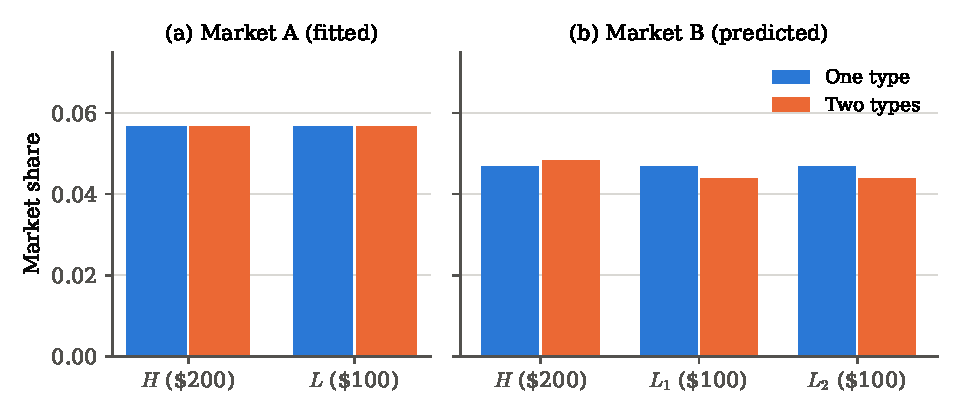
\includegraphics[width=\textwidth]{figures/ch09/twotypes_example.pdf}
\caption{Identifying two types from aggregate shares. Both models fit market A, where the \$200 and
\$100 products have equal shares. In market B, which adds a second \$100 product, the one-type model
predicts three equal shares. The two-type model predicts that the expensive product keeps more of its
share, because the two cheap products compete for the same price-sensitive travelers. Parameters as in
\cref{tab:09-twotypes}.}
\label{fig:09-twotypes}
\end{figure}

\begin{remark}[The role of nesting in the example]\label{rem:09-twotypes-sigma}
The direction of the departure from the one-type prediction depends on the whole specification. With
$\sigma=0$ and the same $\alpha_r$ and $\psi_r$, recalibrating $\xi_H$ to fit market A gives market B
shares of $0.0530$ for $H$ and $0.0576$ for each cheap product. Without nesting, flights compete mainly
with the outside good. Type 2 values every flight highly because $\alpha_2$ is small, so it gives the new
cheap product a larger share than type 1 does, and $H$ loses more. The nesting parameter makes flights
compete with one another within each type. What identifies the types is the existence of departures from
the one-type prediction, and the data determine their direction.
\end{remark}

Random coefficients also change how markups respond to entry. Berry, Carnall and Spiller stress that with
random coefficients, introducing similar products drives markups down \citep[p.~18]{BerryCarnallSpiller2006}.
In \cref{ex:09-twotypes}, the inverse semi-elasticity of $L$'s demand,
$-s_L\big(\frac{\partial s_L}{\partial p_L}\big)^{-1}$, is the markup a single-product seller of $L$ would choose. It falls from $0.453$ (\$45) in market A
to $0.352$ (\$35) in market B, because $L_2$ competes for exactly the travelers who buy $L$. A one-type
nested logit with the same $\sigma$ predicts a fall of only 9\%, which comes from the decline in $L$'s
shares alone.

\subsection{Network costs and economies of density}\label{sec:09-pricing-network}

The cost side of hubbing rests on an engineering argument. Larger aircraft are cheaper to fly per seat
mile, at least on longer routes \citep[pp.~3--4]{BerryCarnallSpiller2006}. For a given flight frequency, a
densely traveled spoke can use larger aircraft. A hub combines passengers bound for many destinations
on one large aircraft to the hub, where they change planes. We first define the relevant cost concepts,
then work through a stylized network, and finally derive the pricing condition of a network carrier.

\begin{definition}[Returns to density and to scale]\label{def:09-rtd}
Let $C(Q,P,w)$ be a carrier's total cost, with traffic $Q$ (for example passenger miles), number of
points served $P$ and input prices $w$. Write $\varepsilon_{CQ}=\frac{\partial\ln C}{\partial\ln Q}$ and
$\varepsilon_{CP}=\frac{\partial\ln C}{\partial\ln P}$. \emph{Returns to density} and \emph{returns to
scale} are
\begin{equation}\label{eq:09-rtd}
RTD=\frac{1}{\varepsilon_{CQ}},\qquad RTS=\frac{1}{\varepsilon_{CQ}+\varepsilon_{CP}} .
\end{equation}
\end{definition}

Returns to density measure the cost of adding traffic to a fixed network, and returns to scale the cost
of expanding traffic and the network together. Since $\varepsilon_{CQ}=\frac{Q}{C}\frac{\partial C}{\partial Q}$, the density elasticity also equals the ratio of marginal to average cost of traffic.
\citet{CavesChristensenTretheway1984} estimate an airline cost function \citep[p.~4]{BerryCarnallSpiller2006}.
Holding the route structure fixed, total cost rises only 80\% as fast as traffic. This means $\varepsilon_{CQ}\approx0.8$ and
$RTD\approx\frac{1}{0.8}=1.25$. Berry, Carnall and Spiller point out two limits of this approach. An
aggregate cost function ignores details of route structure that determine densities. Holding the number
of endpoints fixed, for instance, densities fall as a carrier operates more hubs
\citep[p.~4, n.~7]{BerryCarnallSpiller2006}. And route-level cost data do not exist, since route-level
total or average cost is not even well defined. \citet{BruecknerSpiller1994} instead model the marginal
cost of a passenger on each leg as a function of that leg's density and sum over the legs of an
itinerary. They find that funneling passengers through hub airports raised traffic densities and let
carriers reduce costs \citep[pp.~4--5]{BerryCarnallSpiller2006}. \citet{BruecknerDyerSpiller1992} make
the related point that itineraries through a hub may have lower costs because they raise spoke density
\citep[p.~2]{BerryCarnallSpiller2006}. Berry, Carnall and Spiller adopt the leg-level approach.

\begin{example}[Hub-and-spoke versus point-to-point costs]\label{ex:09-hubcost}
A carrier serves $n$ outer cities and one hub city. Every pair of the $n+1$ cities has $A$ round-trip
passengers. Each leg has cost $C(Q)=aQ^\gamma$ with $0<\gamma\le1$, so legs have \emph{economies of
density}, marginal and average cost falling with traffic, when $\gamma<1$. All legs have equal length and we ignore circuity.

\emph{Point to point.} Every city pair gets a nonstop leg. There are $\frac{n(n+1)}{2}$ legs, each
carrying density $A$, so
\begin{equation*}
C^{PP}=\frac{n(n+1)}{2}\,aA^\gamma .
\end{equation*}

\emph{Hub and spoke.} There are $n$ spokes. The spoke from outer city $e$ carries the $A$ passengers
between $e$ and the hub and the $A$ passengers between $e$ and each of the other $n-1$ outer cities. Its
density is $A+(n-1)A=nA$, so
\begin{equation*}
C^{HS}=n\,a(nA)^\gamma=aA^\gamma\,n^{1+\gamma} .
\end{equation*}

\emph{Comparison.} Dividing,
\begin{equation*}
\frac{C^{HS}}{C^{PP}}=\frac{aA^\gamma n^{1+\gamma}}{\frac{n(n+1)}{2}aA^\gamma}=\frac{2n^\gamma}{n+1} .
\end{equation*}
Hubbing is cheaper if and only if $2n^\gamma<n+1$. With $\gamma=1$ this requires $n<1$, so hubbing is
never cheaper: connecting passengers fly two legs instead of one. With $n=10$ and $\gamma=0.7$ the ratio
is $\frac{2\times10^{0.7}}{11}=\frac{10.02}{11}=0.91$. For $\gamma=0.7$ hubbing lowers total cost once
$n\ge7$, and for $\gamma=0.8$ once $n\ge27$.

\emph{Marginal costs.} Leg marginal cost is $c(Q)=a\gamma Q^{\gamma-1}$. A nonstop passenger in the
point-to-point network costs $a\gamma A^{\gamma-1}$. A connecting passenger in the hub network flies two
spokes of density $nA$ and costs $2a\gamma(nA)^{\gamma-1}$, a ratio of $2n^{\gamma-1}$. A passenger
to or from the hub flies one spoke, a ratio of $n^{\gamma-1}<1$. With $n=10$ and $\gamma=0.7$ the
connecting ratio is $1.00$ and the hub-endpoint ratio is $0.50$.
\end{example}

\begin{figure}[htbp]
\centering
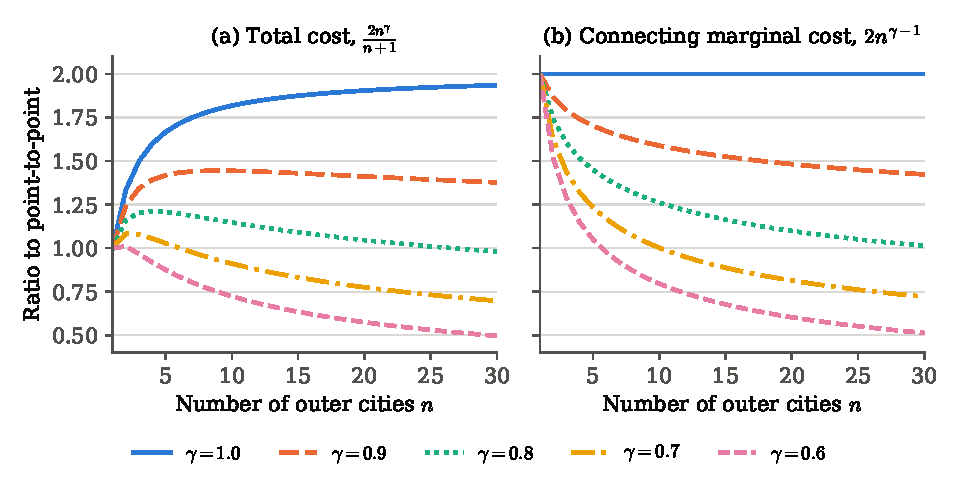
\includegraphics[width=\textwidth]{figures/ch09/hubcost_ratio.pdf}
\caption{Hub-and-spoke relative to point-to-point costs in \cref{ex:09-hubcost}, as functions of the
number of outer cities $n$ for several leg cost elasticities $\gamma$. Panel (a) shows total network cost,
panel (b) the marginal cost of a connecting passenger. Values below the dashed line favor the hub.}
\label{fig:09-hubcost}
\end{figure}

\Cref{fig:09-hubcost} plots both ratios. Three lessons emerge. Economies of density are necessary for a
hub to save cost in this setting, because connecting passengers use two legs. The savings grow with the
size of the network, since each spoke pools more city pairs. And passengers who start or end at the hub
have the lowest marginal cost, because they use one dense spoke. This last point anticipates the finding
of \cref{sec:09-bcs} that carriers with large hubs have lower marginal costs on flights out of their hubs.
The firm-level elasticity of 0.8 is not the same object as the leg-level $\gamma$. If the two were equal,
hubbing would lower total cost in this stylized network only with at least 27 outer cities. The example
ignores the extra distance of connecting trips, the value of frequency, congestion at the hub and the
fact that many thin city pairs would get no nonstop service at all.

\casehead{Itinerary marginal cost}
Let $\mathcal{L}_f$ be the set of legs (spokes) that carrier $f$ flies. As in \cref{sec:09-data},
$\mathcal{L}(j)$ is the set of legs in the itinerary of product $j$. The density $Q_\ell$ of leg $\ell$
counts the passengers on all itineraries that use it, in every market \eqref{eq:09-density}. Legs are
carrier specific, so only carrier $f$'s products contribute to the density of a leg in $\mathcal{L}_f$.
Leg $\ell$ has total cost $C_\ell(Q_\ell,w_\ell)$ and marginal cost
$c_\ell(Q_\ell,w_\ell)=\frac{\partial C_\ell}{\partial Q_\ell}$, where $w_\ell$ collects exogenous leg
characteristics such as distance and airport congestion. Following \citet{BruecknerSpiller1994}, the
marginal cost of product $j$ is the sum of its legs' marginal costs plus a product-specific shock
$\omega_j$:
\begin{equation}\label{eq:09-itin-mc}
mc_j=\sum_{\ell\in\mathcal{L}(j)}c_\ell(Q_\ell,w_\ell)+\omega_j .
\end{equation}
The carrier's total cost is
\begin{equation}\label{eq:09-firm-cost}
C_f=\sum_{\ell\in\mathcal{L}_f}C_\ell(Q_\ell,w_\ell)+\sum_t\ \sum_{j\in\mathcal{J}_f(t)}\omega_jq_j+FC_f ,
\end{equation}
where $FC_f$ is fixed cost. The term $\omega_jq_j$ exists only to give marginal cost an additive error
\citep[p.~13]{BerryCarnallSpiller2006}. Legs are shared by many products, so a product's total cost is
undefined while its marginal cost is well defined. Shared legs create economies of scope across itineraries.
The itinerary New York-Chicago-San Diego shares a spoke with New York-Chicago-Seattle. More demand for New
York-San Diego raises traffic on the New York-Chicago leg \citep[p.~2, n.~5]{BerryCarnallSpiller2006}. With
economies of density, the extra traffic lowers the marginal cost of serving New York-Seattle.

\casehead{The pricing condition of a network carrier}
Assume that demand in market $t$ depends only on the prices of products in market $t$. Using
\eqref{eq:09-firm-cost}, carrier $f$'s profit is
\begin{equation*}
\pi_f=\sum_t\ \sum_{j\in\mathcal{J}_f(t)}(p_j-\omega_j)\,q_j(p)-\sum_{\ell\in\mathcal{L}_f}C_\ell(Q_\ell,w_\ell)-FC_f .
\end{equation*}
Differentiate with respect to the price of a product $j\in\mathcal{J}_f(t)$. Products in other markets do
not respond to $p_j$, so the revenue terms give
$q_j+\sum_{k\in\mathcal{J}_f(t)}(p_k-\omega_k)\frac{\partial q_k}{\partial p_j}$. The cost terms give
$-\sum_{\ell\in\mathcal{L}_f}c_\ell(Q_\ell,w_\ell)\frac{\partial Q_\ell}{\partial p_j}$, with
\begin{equation*}
\frac{\partial Q_\ell}{\partial p_j}=\sum_{k\in\mathcal{J}_f(t):\,\ell\in\mathcal{L}(k)}\frac{\partial q_k}{\partial p_j}.
\end{equation*}
Exchanging the order of summation over legs and products,
\begin{equation*}
\sum_{\ell\in\mathcal{L}_f}c_\ell\sum_{k\in\mathcal{J}_f(t):\,\ell\in\mathcal{L}(k)}\frac{\partial q_k}{\partial p_j}
=\sum_{k\in\mathcal{J}_f(t)}\frac{\partial q_k}{\partial p_j}\sum_{\ell\in\mathcal{L}(k)}c_\ell .
\end{equation*}
Collecting terms and using \eqref{eq:09-itin-mc},
\begin{equation}\label{eq:09-network-foc}
\frac{\partial\pi_f}{\partial p_j}
=q_j+\sum_{k\in\mathcal{J}_f(t)}\Big[p_k-\omega_k-\sum_{\ell\in\mathcal{L}(k)}c_\ell(Q_\ell,w_\ell)\Big]\frac{\partial q_k}{\partial p_j}
=q_j+\sum_{k\in\mathcal{J}_f(t)}(p_k-mc_k)\frac{\partial q_k}{\partial p_j}=0 .
\end{equation}
This is the condition of \citet[p.~15]{BerryCarnallSpiller2006}.

Equation \eqref{eq:09-network-foc} has the same form as the single-market condition behind
\eqref{eq:09-fm-markup}. The network enters only through the level of each $mc_k$, evaluated at
network-wide equilibrium densities. A lower price in market $t$ raises density on the legs its products
share with other markets. With economies of density this lowers the marginal cost of the carrier's
products elsewhere, and those products are repriced in turn. Equilibrium prices are therefore linked
across all markets that share legs, even though each first-order condition involves one market only. For
estimation, \eqref{eq:09-fm-markup} and \eqref{eq:09-itin-mc} combine into
$p_j-\text{markup}_j(\theta_d)=\sum_{\ell\in\mathcal{L}(j)}c_\ell(Q_\ell,w_\ell)+\omega_j$, a regression of
price net of markup on leg cost terms.

Densities are endogenous in that regression. A product with high unobserved demand $\xi$ raises the
density of its legs, which lowers marginal cost when there are economies of density. Demand shocks thus
move density and price together, and shocks to $\omega$ may be correlated across products that share
legs. Estimation must instrument for density with variables that shift traffic on a leg but not product
costs. Berry, Carnall and Spiller use population and network characteristics of the endpoint cities
(\cref{sec:09-bcs}).

\begin{remark}[Markups are not profits]\label{rem:09-markups-profits}
Let a leg have cost $C_\ell(Q)=F_\ell+aQ^\gamma$ with $F_\ell\ge0$ and $\gamma<1$. Average cost is
$\frac{F_\ell}{Q}+aQ^{\gamma-1}$ and marginal cost is $\gamma aQ^{\gamma-1}$, so
\begin{equation*}
AC-MC=\frac{F_\ell}{Q}+(1-\gamma)aQ^{\gamma-1}>0 .
\end{equation*}
Pricing at marginal cost loses $Q(AC-MC)=F_\ell+(1-\gamma)aQ^\gamma$. At the break-even price $p=AC$, the
Lerner index is $1-\frac{MC}{AC}$. With $F_\ell=0$ this equals $1-\gamma$. More generally, at $p=AC$ the
Lerner index is $1-\varepsilon_{CQ}=1-\frac{1}{RTD}$, so a density elasticity of 0.8 implies a
break-even markup of 20\% of price. Positive markups over marginal cost are thus consistent with zero
economic profit. Berry, Carnall and Spiller warn that airlines may be unprofitable even with large
markups \citep[p.~16]{BerryCarnallSpiller2006}. Fixed costs may be large, and marginal cost may decline
over a wide range of output. The contestability prediction (C4) of \cref{sec:09-contest}
must be read with this in mind. Markups signal market power only when they exceed what is needed to cover
the gap between average and marginal cost.
\end{remark}

The theory of this section organizes the evidence that follows. The conduct model of
\cref{sec:09-pricing-conduct} and its umbrella term frame Borenstein's regressions in
\cref{sec:09-borenstein}. \Cref{prop:09-dominance} predicts the asymmetry he finds between dominant
carriers and their rivals. The finite-mixture model, its markup formula \eqref{eq:09-fm-markup} and the
network cost structure \eqref{eq:09-itin-mc} are the model that Berry, Carnall and Spiller take to data in
\cref{sec:09-bcs}.
